

\begin{center}

\justifying
\chapter{\large PROJECT DESIGN}

\justifying
\section{\normalsize DATAFLOW DIAGRAM LEVEL 0}
\hspace{5mm} A data flow diagram (DFD) is a graphical representation of the "flow" of data through an information system, modeling its process aspects. Often they are a preliminary step used to create an overview of the system which can later be elaborated. DFDs can also be used for the visualization of data processing (structured design.\\
\hspace{5mm} DFD shows interaction between external entities and processes and process and data store.\\
%\\ \hspace*{1cm} Following is the Dataflow diagram level 0
\begin{figure}[H]
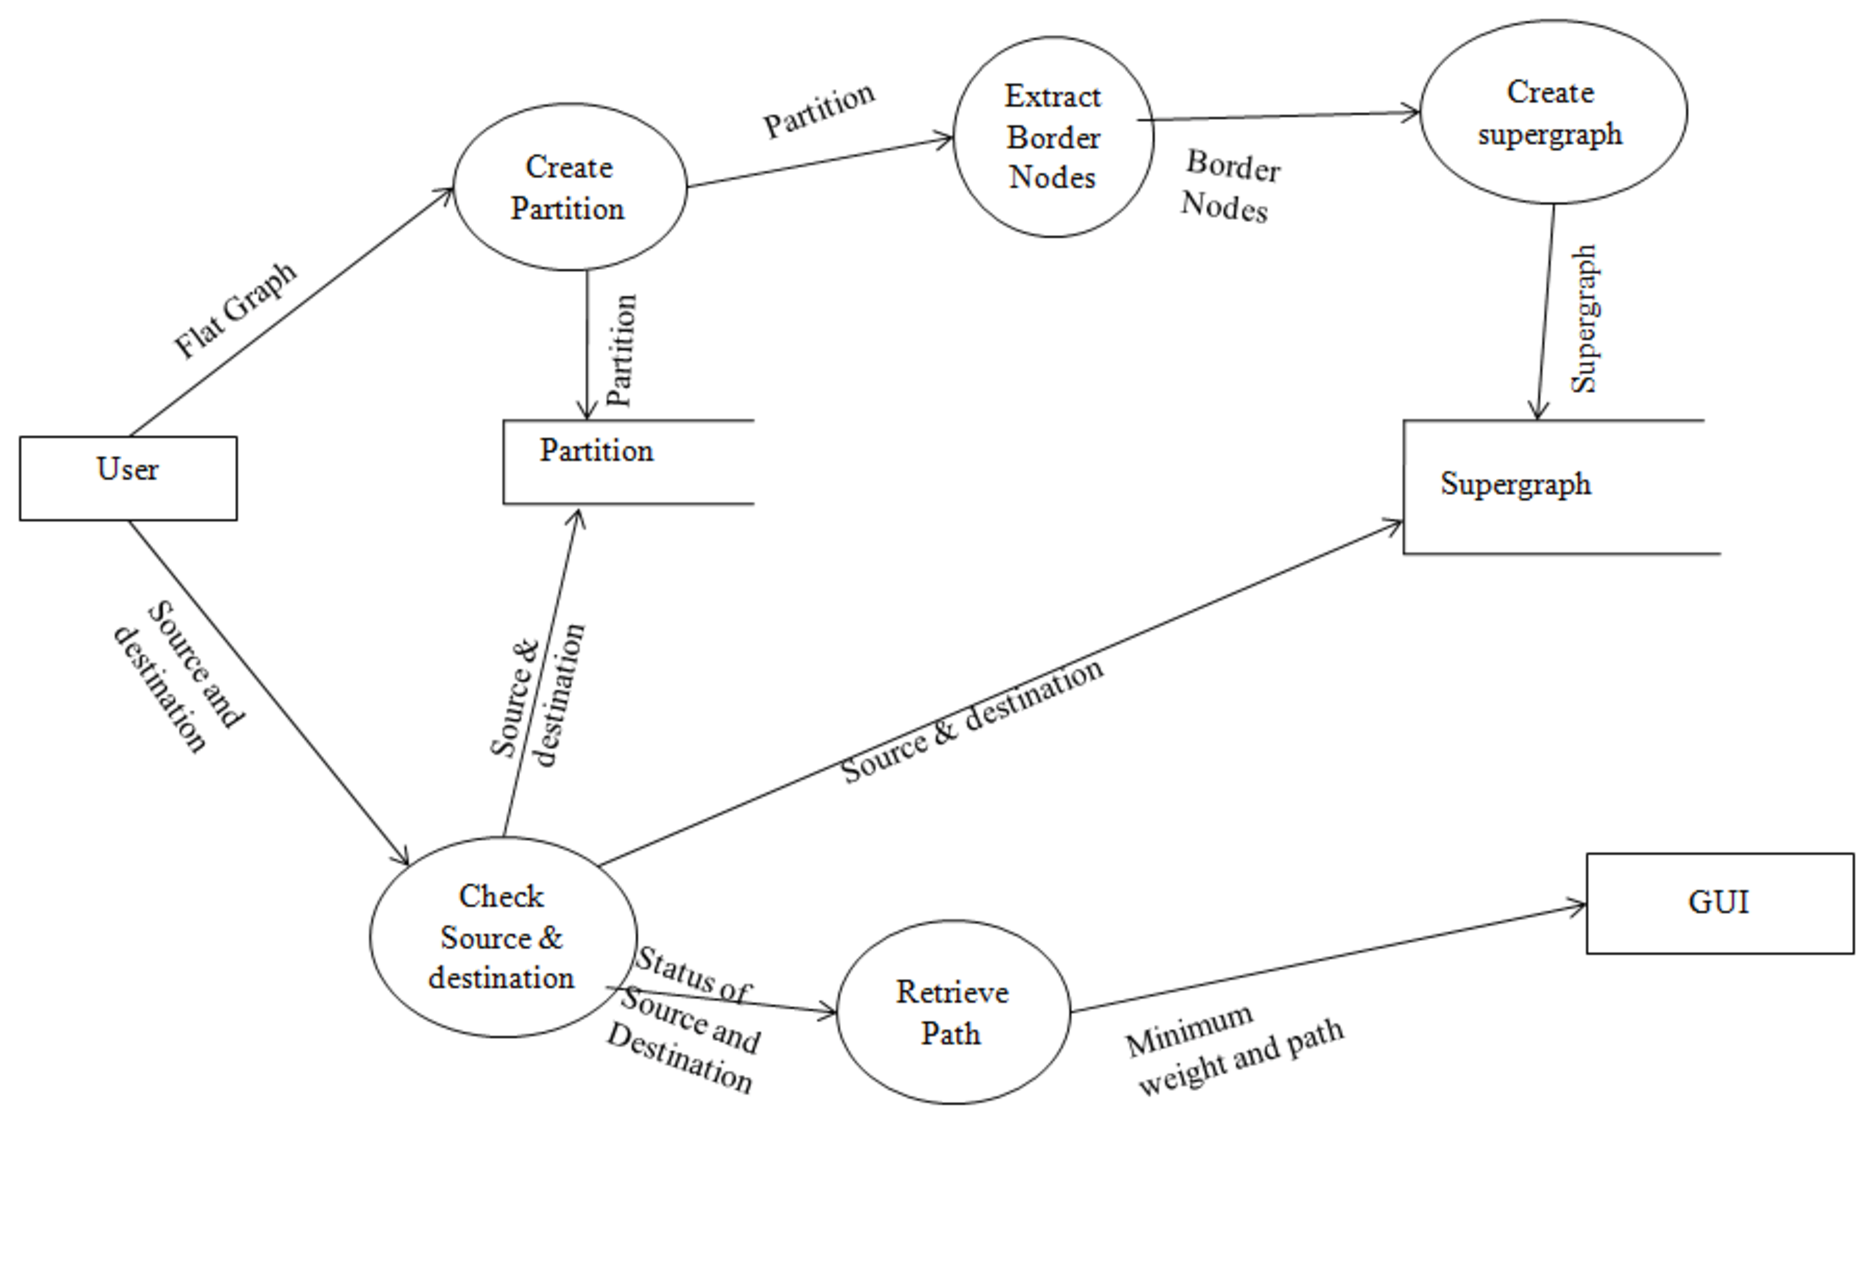
\includegraphics[width=16cm,height=10cm]{DFD.eps}
\caption{Data Flow Diagram}
\end{figure}
\newpage


\section{\normalsize ENTITY-RELATIONSHIP DIAGRAM}
\hspace{5mm} Following is the Entity Relationship Diagram which shows relationship between different entities.
\begin{figure}[H]
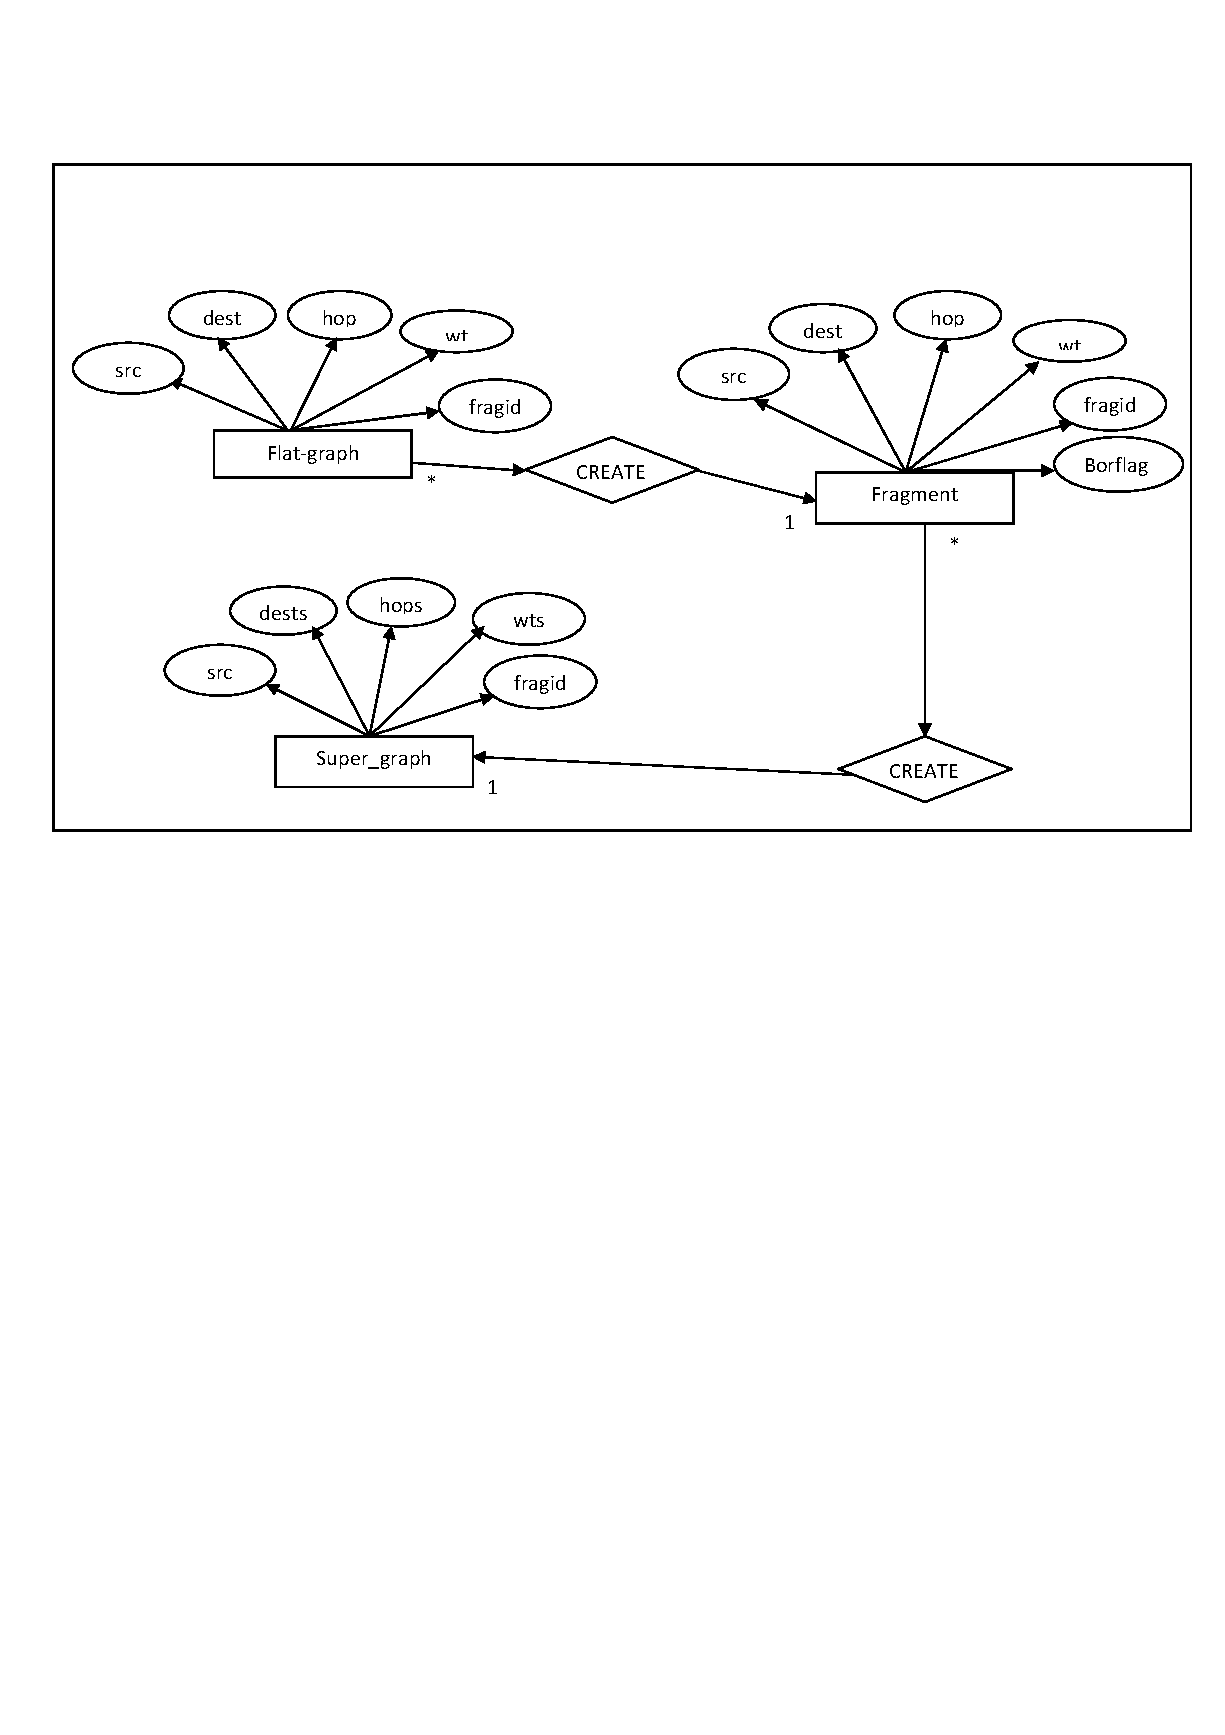
\includegraphics[width=16cm,height=15cm]{ER1.eps}
\caption{Entity-Relationship Diagram}
\end{figure}


\newpage




\section{\normalsize CLASS DIAGRAM}
\hspace*{5mm} The below diagram depicts the class diagram for image processing. System will comprise of various classes such as image, cartoon, imagesketch etc. The class diagram shows interdependency between the classes and how they communicate between them.\\
\begin{figure}[H]
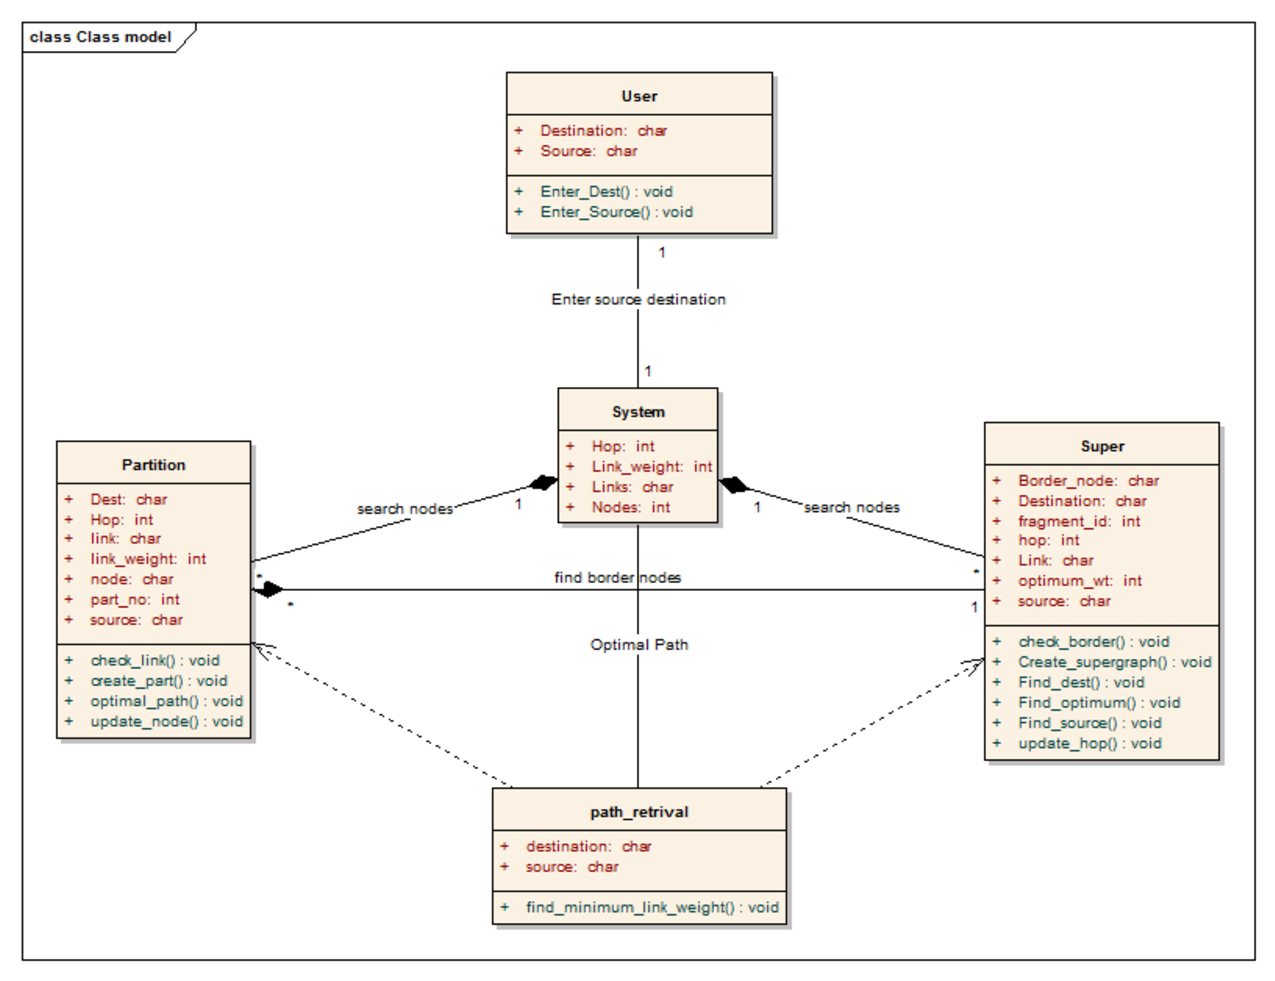
\includegraphics[width=17cm,height=17cm]{Class.eps}
\caption{Class Diagram}
\end{figure}
\newpage


\section{\normalsize SEQUENCE DIAGRAM}
\hspace{5mm} Sequence diagram represents the dynamic behaviour of the system. A Sequence diagram is a structured representation of behaviour as a series of sequential steps over time. The application’s sequence diagram shows how the elements of the application pass messages to each other during actual execution.\\
%\\ \hspace*{1cm} Following shows Sequence Diagram 
\begin{figure}[H]
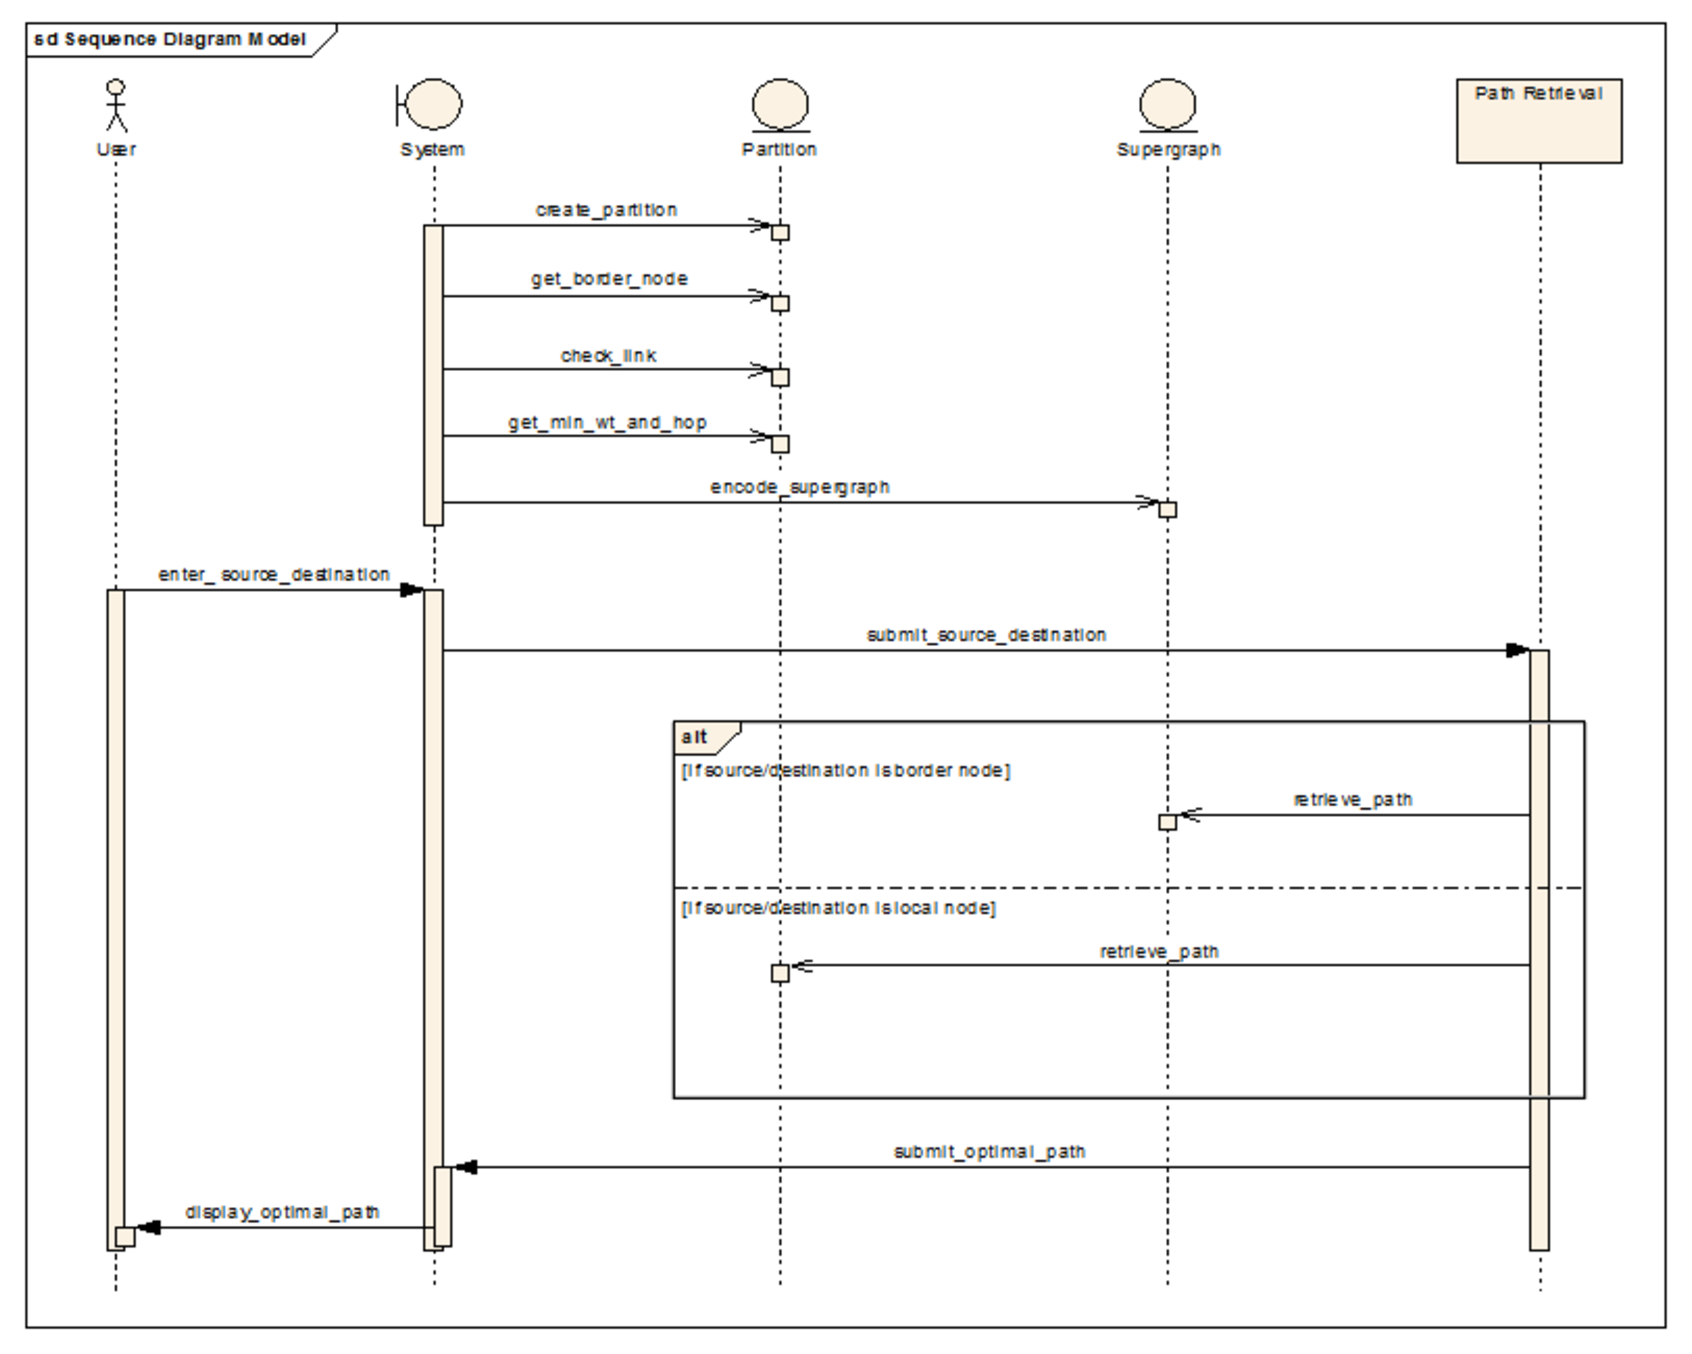
\includegraphics[width=17cm,height=17cm]{seq.eps}
\caption{Sequence Diagram}
\end{figure}
\newpage

\section{\normalsize COLLABORATION DIAGRAM}
\hspace{5mm} Following is the Collaboration diagram which shows the communication between different entities.
\begin{figure}[H]
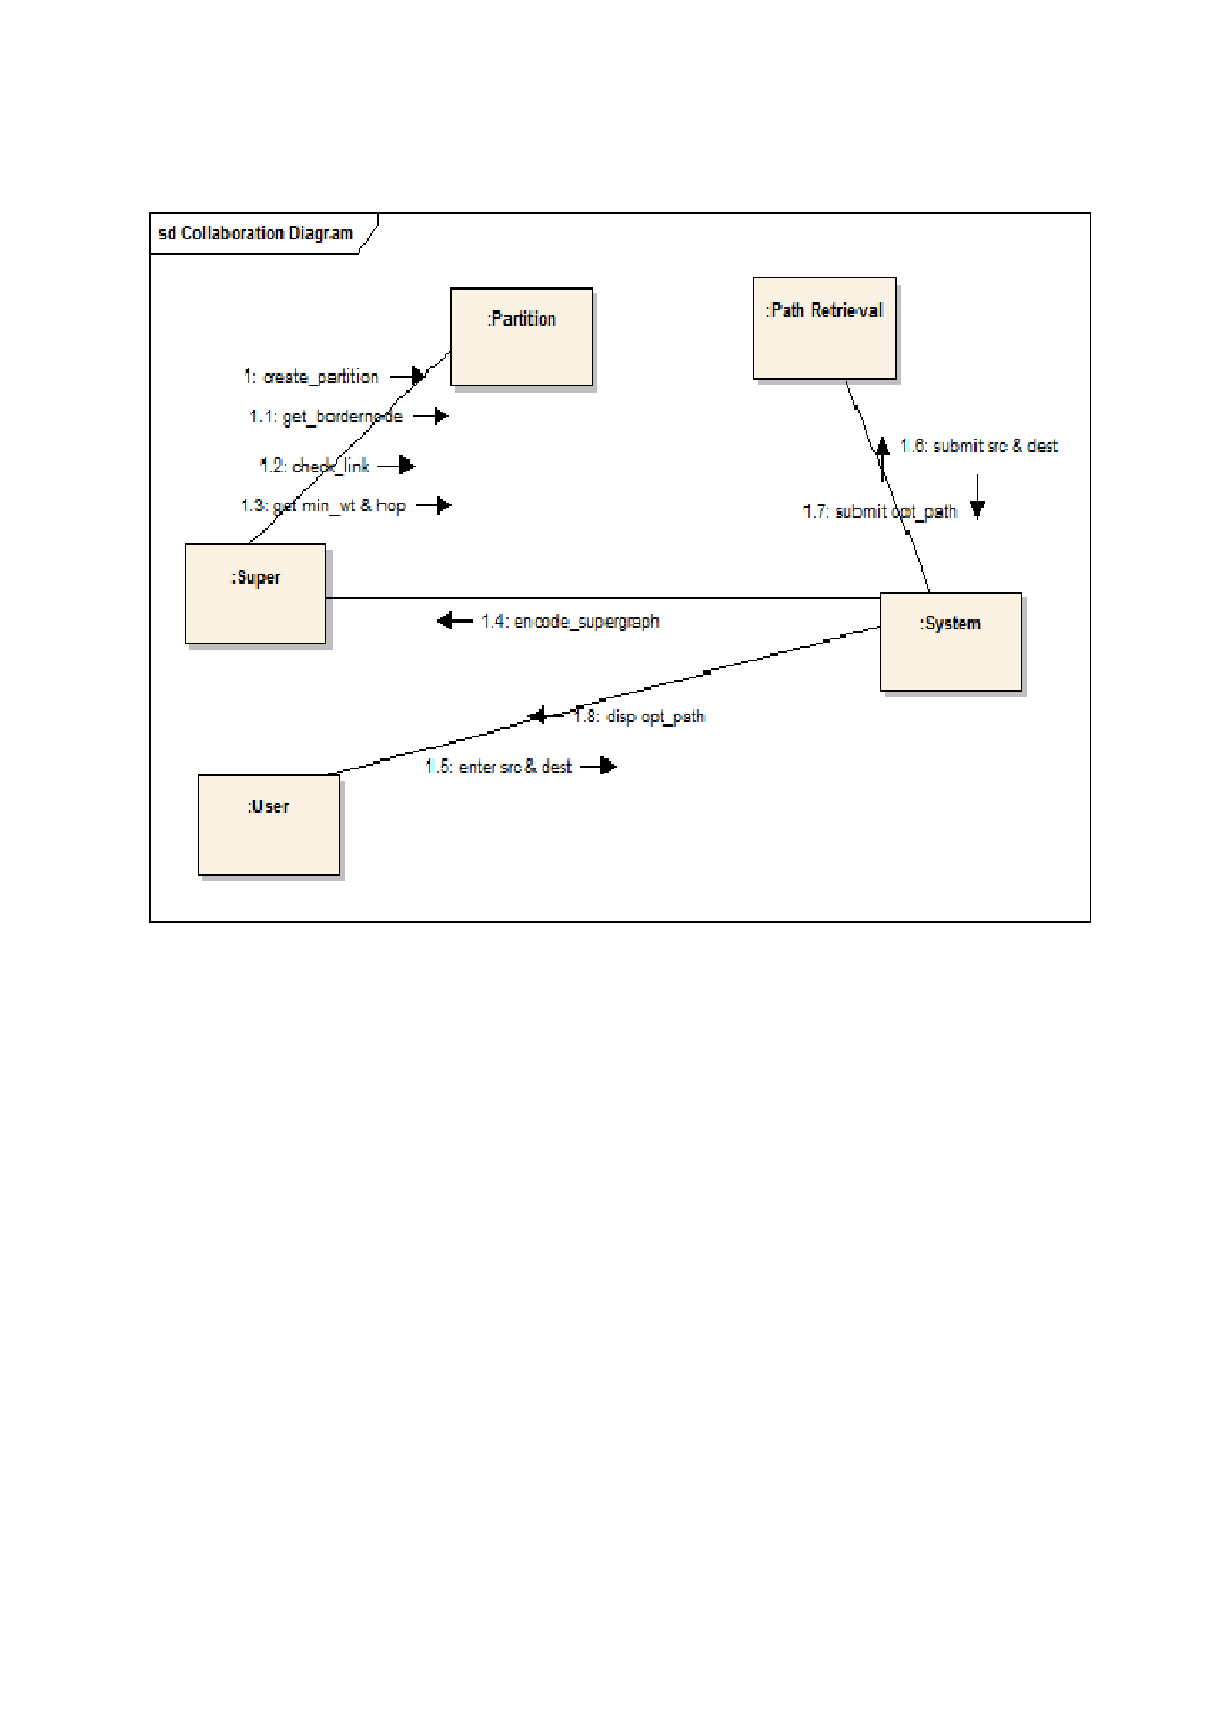
\includegraphics[width=14cm,height=20cm]{coll.eps}
\caption{Collaboration Diagram}
\end{figure}
\newpage



\section{\normalsize STATE TRANSITION}
\hspace{5mm} This diagram is a way of describing the time-dependent behavior of a system. State diagrams are used to describe the behavior of a system.  State diagrams describe all of the possible states of an object as events occur.  Each diagram usually represents objects of a single class and tracks the different states of its objects through the system.\\
%\\ \hspace*{1cm} Following is the State Transition diagram 
\begin{figure}[H]
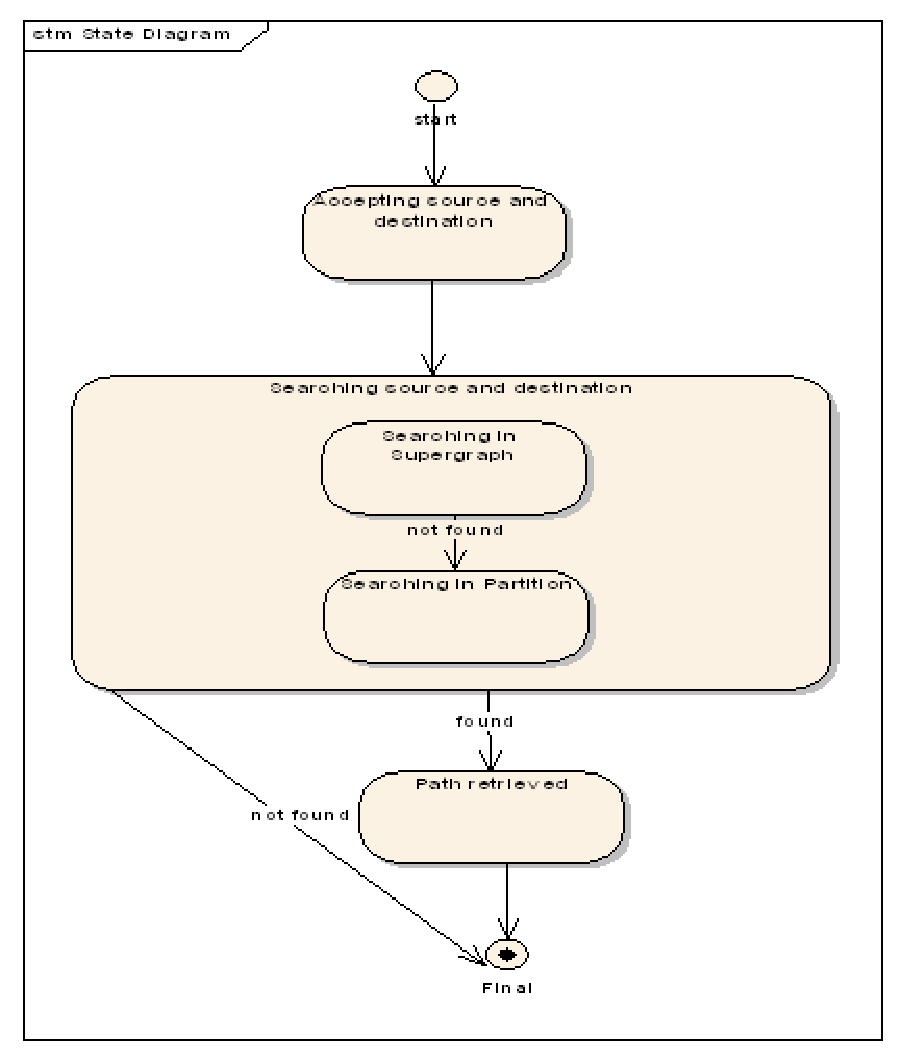
\includegraphics[width=14cm,height=17cm]{state.eps}
\caption{State Transition Diagram}
\end{figure}
\newpage


\section{\normalsize DEPLOYMENT DIAGRAM}
\hspace{5mm} A deployment diagram in the Unified Modeling Language models the physical deployment of artifacts on nodes.
\begin{figure}[H]
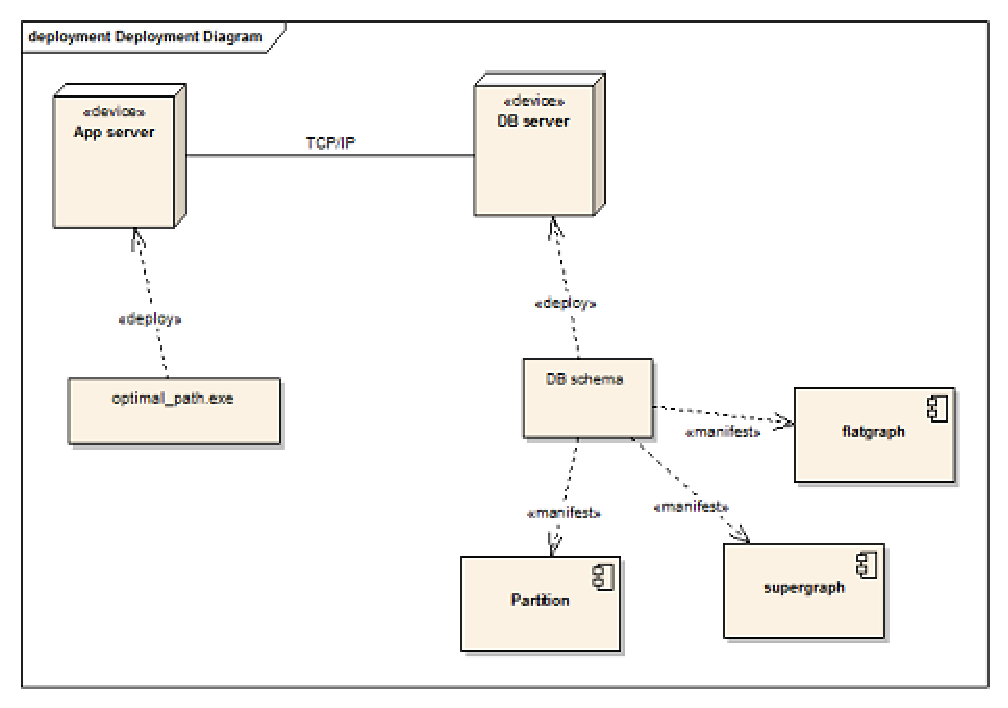
\includegraphics[width=17cm,height=17cm]{dep.eps}
\caption{Deployment Diagram}
\end{figure}
%\newpage



\end{center}